\section{Markov Chain Monte Carlo}
\subsection{Introduction to Markov Chains}
In most cases, we assume the samples are independent. However, it is a poor assumption as this may rarely happen in reality. Therefore, we assume the data are dependent and hence we have \textbf{sequential data}. More specifically, we can use \textbf{markov chain} to model the sequential data.
\begin{figure}[H]
    \centering
    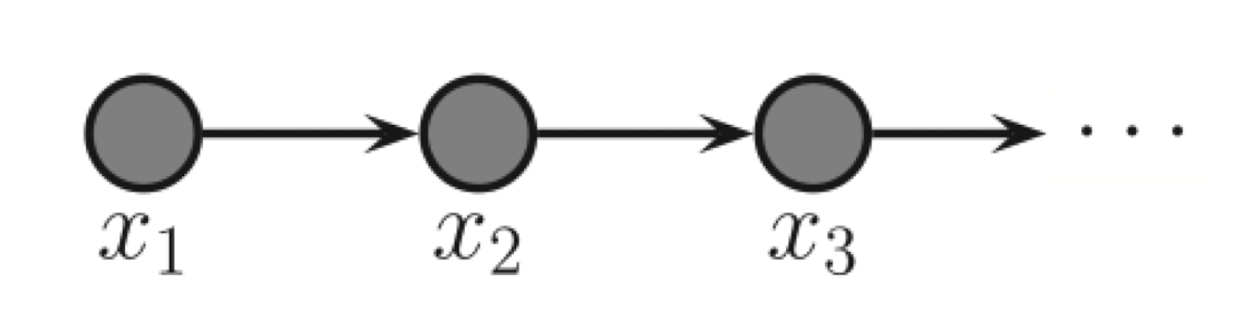
\includegraphics[width = .6\linewidth]{figures/section6/figure_6_1.png}
    \caption{First order Markov Chain}
    \label{fig:f_mc}
\end{figure}
\hyperref[fig:f_mc]{Figure 6.1} shows an example of First order Markov chain.
\begin{align*} 
    p\left(x_t | x_{1: t-1}\right)&=p\left(x_t | x_{t-1}\right)\\
    &=\prod_{t=1}^T p\left(x_t | x_{t-1}\right)
\end{align*}
From the graph, we can see that the first order means each node is conditioned on the previous node. We can therefore generalize to higher order Markov Chains.
\begin{itemize}    \item For second-order Markov Chains:
    $$p\left(x_t | x_{1: t-1}\right)=p\left(x_t | x_{t-1},x_{t-2}\right)$$
    \item For m-order Markov Chains:
    $$p\left(x_{1: T}\right)=p\left(x_t | x_{t-1:t-m}\right)$$
\end{itemize}
We have two further definations:\\
\textbf{Stationary(homongeneous) Markov Chain}: The distribution generating the data does not change over time:
$$p(x_{t+1}=y|x_t=x)=p(x_{t+2}=y|x_{t+1}=x)$$ 
\textbf{Non-stationary Markov Chain}: $p(x_{t+1}=y|x_t=x)$ depends on time $t$.

\subsubsection*{Transition Matrix}
If we assume $x_t$ is discrete: $x_t\in\{1,2,\cdots,K\}$. Then the conditional distribution $p(x_t|x_{t-1})$ can be written as a $K\times K$ matrix, which is called the \textbf{transition (stochastic) matrix $A$}. Each element on $A$ represents the probability of transition from $t-1$ to $t$, i.e.
$$A_{ij}=p(x_t=j|x_{t-1}=i),\:A\in K\times K$$
We also have:
\begin{align*} 
    p\left(x_t=j\right) & =\sum_i p\left(x_t=j | x_{t-1}=i\right) p\left(x_{t-1}=i\right) \\ 
    & =\sum_i A_{i j} p\left(x_{t-1}=i\right)
\end{align*}
The sum for each row in $A$ equals to \textbf{1} as it represent all the possibilities of changing from $t-1$ to $t$ ginve $i$ at $t-1$.
$$\sum_i A_{i j}=1$$
\textit{An example of transition matrix can be found \hyperref[fig:transition-example]{here}.}\\
The $n$-step transition matrix $A(n)$is the probability of transferring from two states in $n$ steps, where $n$ can be considered as \textit{"n"} times. In equation:
$$
A_{i j}(n)=p\left(x_{t+n}=j | x_t=i\right)
$$
Since the one-step transition matrix considers $t-1$ and $t$ (or equivalently $t$ and $t+1$)
$$A(1)=A$$
\textbf{Chapman-Kolmogorov equations}:
\begin{align*}
    A_{i j}(m+n)&=\sum_{k=1}^K A_{i k}(m) A_{k j}(n)\\
    \Leftrightarrow A(m+n)&=A(m) A(n)
\end{align*}

It says we can find an intermediate state $k$ between $i$ and $j$, which takes $m$ steps from $i$ to $k$, and $n$ steps from $k$ to $j$. It is similar to lattice paths on combinatorics.\\
$\Rightarrow A(n)=A(1+n-1)=A \cdot A(n-1)=A \cdot A \cdot A(n-2)=\cdots=A^n$.

\subsubsection*{Markov Language Models}
Language models can be represented as Markov Chains. That said, each word is a state, and the probability of transition from one word to another can be also represented as transition matrix.

\begin{align*} 
    p\left(x_{1: T} | \theta\right) & =\pi\left(x_1\right) A\left(x_1, x_2\right) \cdots A\left(x_{T-1}, x_T\right) \\
    & =\underbrace{\prod_{j=1}^K \pi_j^{1\left[x_1=j\right]}}_{\text{prob. starting with }x_1} \prod_{t=2}^T \prod_{j=1}^K \prod_{k=1}^K A_{j k}^{1\left[x_t=k, x_{t-1}=j\right]}
\end{align*}

\subsection{Stationary distribution of a (homongeneous) Markov Chain}
The stationary\footnote{the "stationary" in "stationary distribution" is not as same as in "stationary Markov chain." Therefore, we usually called it as homongeneous Markov chains.} distribution is the \textbf{long-term} distribution over states. It is also called the \textbf{steady state}. In notation, we have $\pi_t(j)=p(x_t=j)$, to be the probability of being in state $j$ on time $t$.\\
\begin{itemize}
    \item We have the initial distribution which is given by $\pi_0\in\mathbb{R}^{K}$
    \item We then represent $\pi_1$ as:
    $$\pi_1(j)=\sum_{i=1}^K p\left(x_1=j | x_0=i\right) \pi_0(i)=\sum_{i=1}^K A_{i j} \pi_0(i)=\sum_{i=1}^K\left(A^{\top}\right)_{j i} \pi_0(i)$$
    $$\Rightarrow \pi_1=A^T\pi_0$$
    \item We can therefore generalize to $\pi_t$.
    $$\pi_t=A^{\top} \pi_{t-1}=A^{\top} A^{\top} \pi_{t-2}=\cdots=\left(A^{\top}\right)^t \pi_0$$
    \item If we do this for many steps; eventually, the distribution of $\pi_t$ may converge:
    $$\pi=A^T\pi$$
    which is the stationary distribution of the Markov chain.
\end{itemize}

\textbf{Recall: Eigenvalues and Eigenvectors}\\
Let $T$ be a transformation, $\mathbf{v}$ be a vector and $\lambda$ be a constant. If we have:
$$T\mathbf{v}=\lambda\mathbf{v}$$
Then $\mathbf{v}$ is the eigenvector of $T$ and $\lambda$ is the eigenvalue.\\

Therefore, it follows that the statioanary distribution $\pi$ is an eigenvector of $A^T$ with eigenvalue 1. In other words, $A$ and $A^T$ have the same eigenvalues and $A\mathbf{1}=\mathbf{1}$ as the row sum of $A$ is 1. Thus, due to the equality of characteristics polynomials, 1 is also the eigenvalue of $A^T$. More importantly, \colorbox{yellow}{\textbf{stationary distribution is NOT unique}}.\\

\textit{An example of how to compute the stationary distribution can be found here}.

\subsubsection*{Detailed balance equation}
Markov Chain is called:
\begin{itemize}
    \item \textbf{irreducible} if we can get from any state to any other state.
    \item \textbf{regular} if $A^n$ has positive entries for some $n$.
    \item \textbf{time reversible} if there exists a distribution $\pi$ such that
    $$
    \underbrace{\pi_i A_{i j}=\pi_j A_{j i}}_{\textbf{detailed balance equation}} \quad \text { for all } i, j .
    $$
    In other words, detailed balance means the probability of transition from one state to another and reverse back is \textbf{equally possible}.
\end{itemize}
\begin{theorem}
    If a markov chain with transition matrix $A$ satisfies the detailed balance with respect to distribution $\pi$, then $\pi$ is a stationary distribution.
\end{theorem}
Recall in rejection sampling, we accept the samples independently. In contrast, we assume the samples are \textbf{dependent}, where each sample is a state in the Markov chain and $x^{(t)}$ has a probability distribution depending on the previous one $x^{t-1}$. In other words, we will \textbf{learn} from the previous samples. Hence the stationary distribution will be $p(x)$.\\

\subsection{Metropolis-Hasting Algorithms}

Compared to rejection sampling, metropolis-hasting prose a simple density $q$ which depends on the current state $x^{(t)}$. If $q$ is Gaussian, then its center will be $x^{(t)}$. As before, assume we can evaluate $\tilde{p}(x)$ for any $x$. The algorithm follows as:
\begin{itemize}
    \item We firstly have a tentative new state $x^{\prime}$ is generated from the proposal density $q\left(x^{\prime} | x^{(t)}\right)$. We accept the new state with probability
    \item We then compute:
    $$
    A\left(x^{\prime}|x^{(t)}\right)=\min \left\{1, \underbrace{\frac{\tilde{p}\left(x^{\prime}\right) q\left(x^{(t)}|x^{\prime}\right)}{\tilde{p}\left(x^{(t)}\right) q\left(x^{\prime} | x^{(t)}\right)}}_{\mathcal{B}}\right\}
    $$
    \item for $\mathcal{B}$
    \begin{itemize}
        \item If $\mathcal{B}>1$, then accept the new state.
        \item If $\mathcal{B}<1$, we sample $u\sim N(0,1)$. Accept if $u\leq\mathcal{B}$;otherwise reject.
    \end{itemize}
\end{itemize}
-Metropolis: Simpler version when $q\left(x^{\prime} | x\right)=q\left(x \mid x^{\prime}\right)$ for all $x, x^{\prime}$.
\begin{theorem}
    This procedure defines a Markov chain with stationary distribution $\pi(x)$ equal to the target distribution $p(x)$. $\pi(x)=p(x)$. \textit{proof \hyperref[sec:proof-metro]{here}}
\end{theorem}
